% begin module parametric-intro
\begin{frame}
\frametitle{(11.1)  Curves Defined by Parametric Equations}
\begin{columns}[c]
\column{.4\textwidth}
\ \only<handout:0| -1>{%
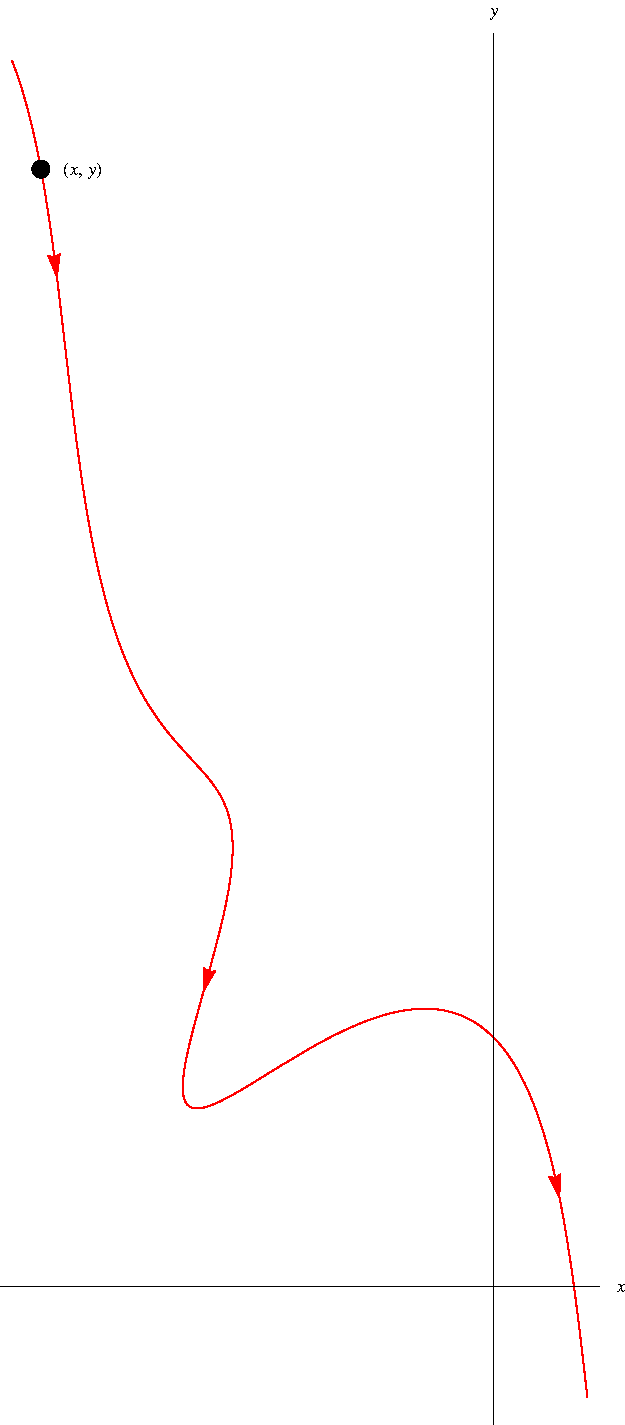
\includegraphics[height=7cm]{parametric-curves/pictures/11-01-parametrica.pdf}%
}%
\only<handout:0| 2>{%
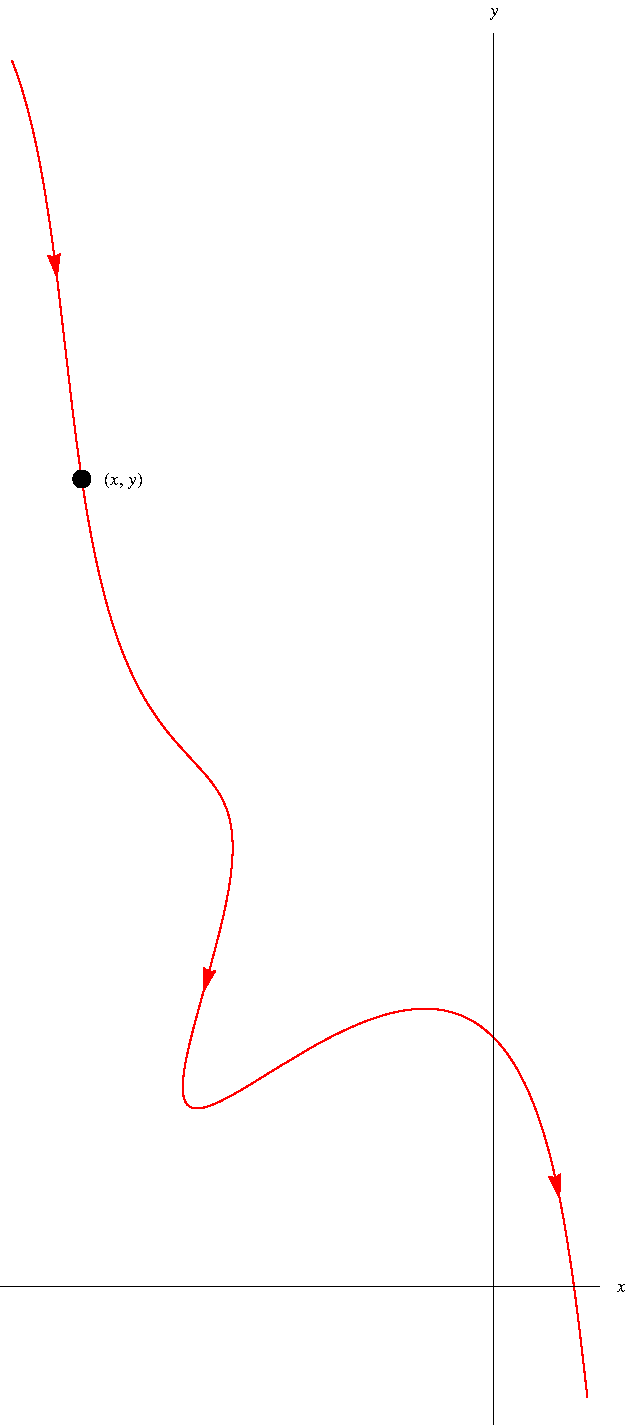
\includegraphics[height=7cm]{parametric-curves/pictures/11-01-parametricb.pdf}%
}%
\only<handout:0| 3>{%
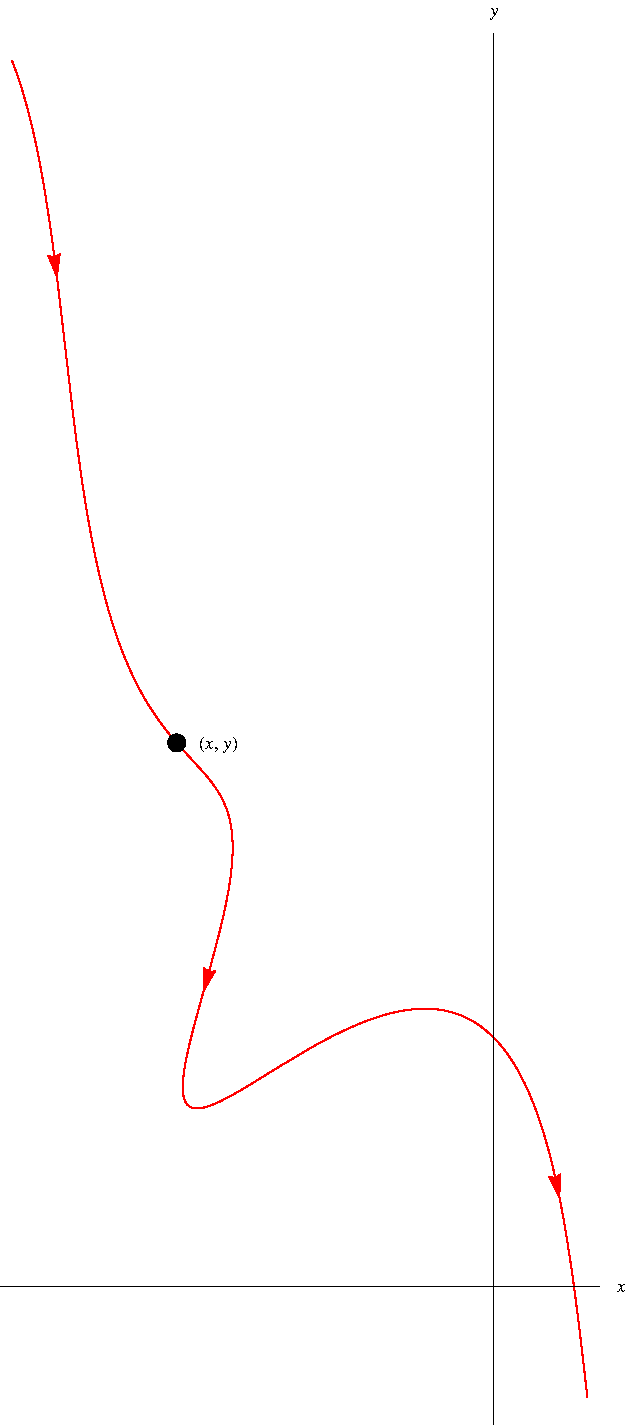
\includegraphics[height=7cm]{parametric-curves/pictures/11-01-parametricc.pdf}%
}%
\only<handout:0| 4>{%
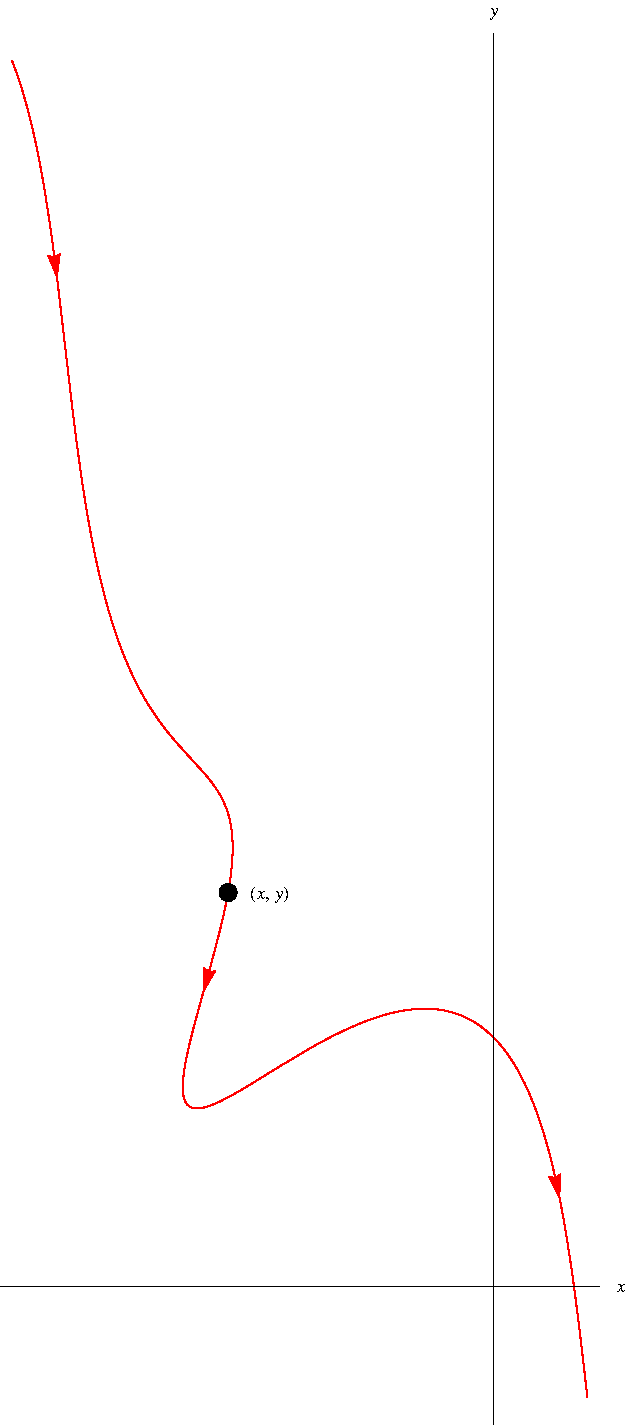
\includegraphics[height=7cm]{parametric-curves/pictures/11-01-parametricd.pdf}%
}%
\only<handout:0| 5-7>{%
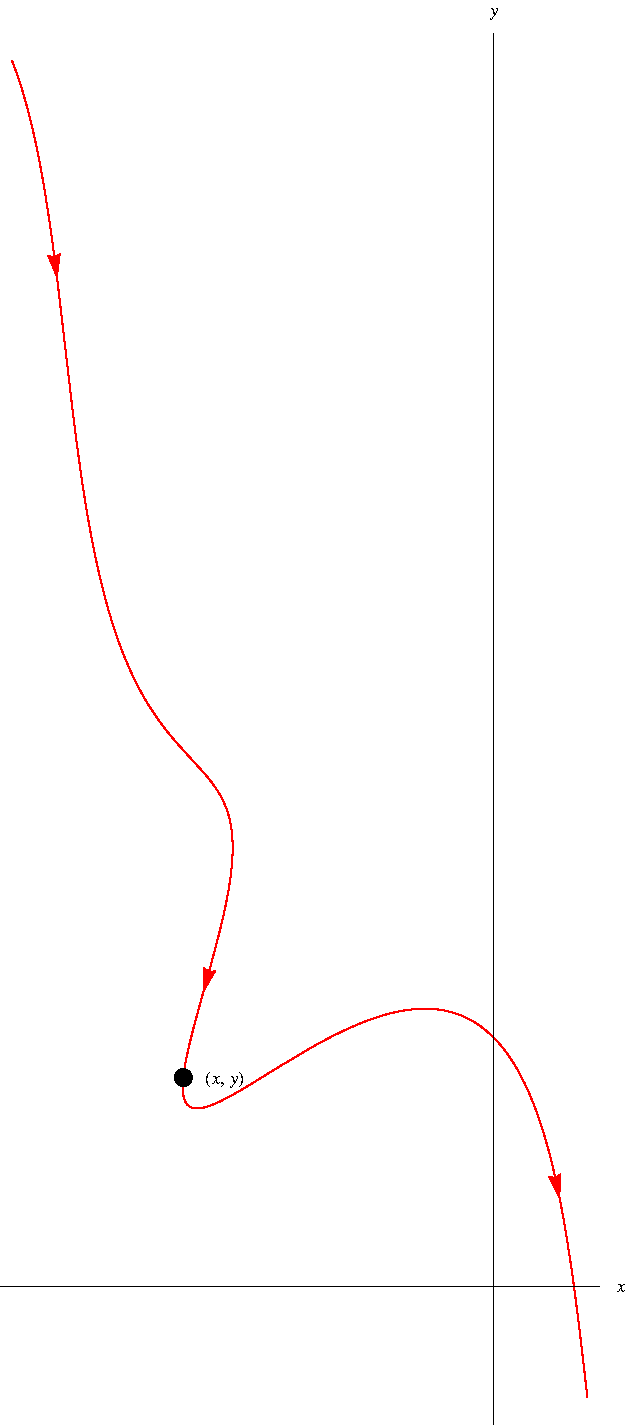
\includegraphics[height=7cm]{parametric-curves/pictures/11-01-parametrice.pdf}%
}%
\only<8->{%
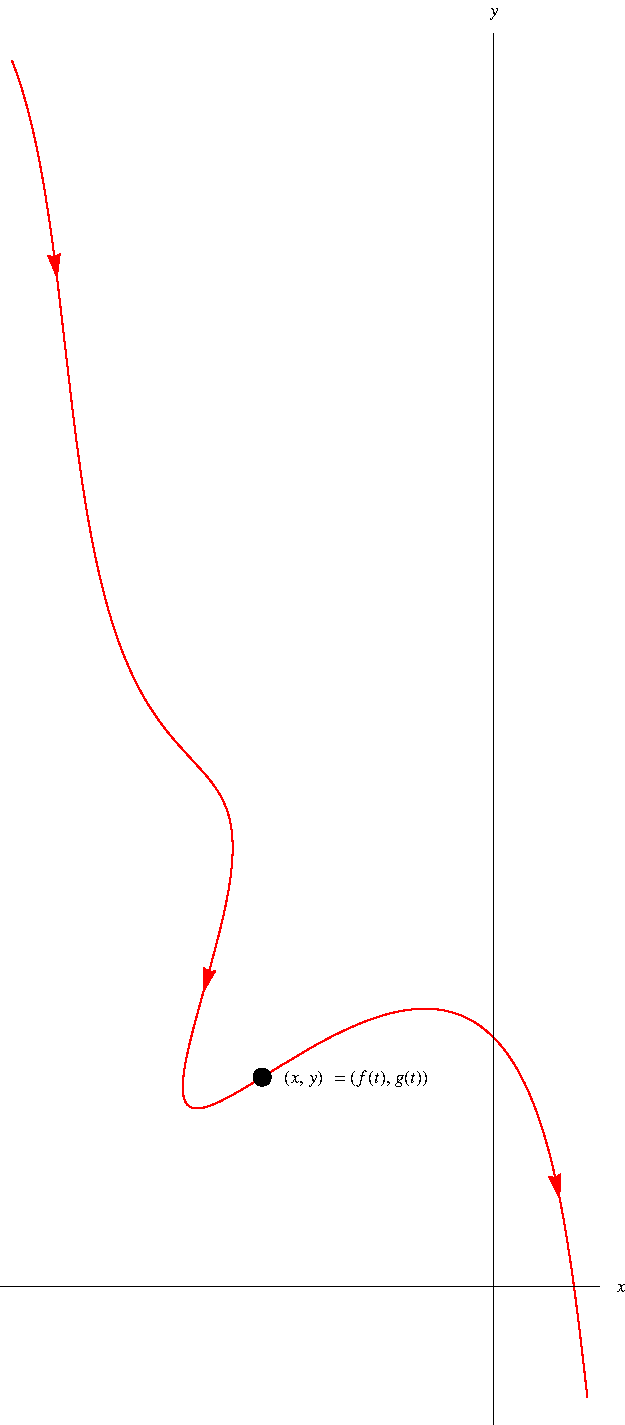
\includegraphics[height=7cm]{parametric-curves/pictures/11-01-parametricf.pdf}%
}%
\column{.6\textwidth}
\begin{itemize}
\item  Suppose a particle moves along the curve in the picture.
\item<6->  We can't write the curve as $y = f(x)$ because it fails the vertical line test.
\item<7->  But the $x$-coordinate and $y$-coordinate of the particle are functions of the time $t$.
\item<8->  We can write $x = f(t)$ and $y = g(t)$.
\item<9->  These are called parametric equations, and the curve is called a parametric curve.
\end{itemize}
\end{columns}
\end{frame}
% end module parametric-intro
